% PROGETTAZIONE E CODIFICA

\chapter{Progettazione e codifica}

\section{Progettazione ed implementazione delle API}

\subsection{Descrizione dell'architettura}

Dato l'utilizzo dell'architettura \textit{serverless}, non si è applicato nella
scrittura delle API alcun tipo particolare di \textit{pattern}. L'architettura
di tipo \textit{serverless} infatti definisce in modo chiaro la delegazione
delle varie responsabilità a componenti molto piccoli e ben definiti. Questo
inoltre permette di avere tempi di risposta molto brevi.
La parte dedicata alla interazione con gli utenti è stata chiamata
\textit{webhook} a livello progettuale, per distinguerla dalle API.

\subsection{Descrizione delle API}
Come già accennato nella sezione \ref{prj:serverless:api}, le funzionalità più
importanti sono state suddivise in differenti API, ognuna delle quali risiede
in una propria istanza di AWS Lambda.

Comparando questa architettura con un classico pattern \textbf{MVC}, queste API
corrisponderebbero al \textit{Model}, che si occupa di gestire parti della
logica della applicazione. Essendo queste parti costituite da una sola
responsabilità e con un solo compito, la loro implementazione si è
concretizzata nella realizzazione di una sola classe per API.

\section{Descrizione del \textit{webhook}}
La parte dedicata all'interazione con gli utenti è stata realizzata sempre
usando l'architettura \textit{serverless}, ma essendo la sua complessità
maggiore la strutturazione a classi è stata necessaria al fine di mantenere una
facile comprensione del programma e una buona estendibilità. Tuttavia, per la
natura del servizio che PastBot ricopre, si è scelto di usare una modellazione
ad eventi per gestire le richieste provenienti dalla piattaforma Facebook
Messenger. In base agli eventi che vengono gestiti PastBot si occupa di fare le
chiamate alle API corrette. Comparandolo con il pattern di tipo \textbf{MVC},
\textit{webhook} si occupa di ricoprire la \textit{View} e il
\textit{Controller}.

\section{Descrizione delle classi}
Di seguito si eseguirà una descrizione delle classi più significative che
compongono PastBot e le relative API, suddivise in base alla componente alla
quale appartengono.

\begin{figure}[H]
  \centering
  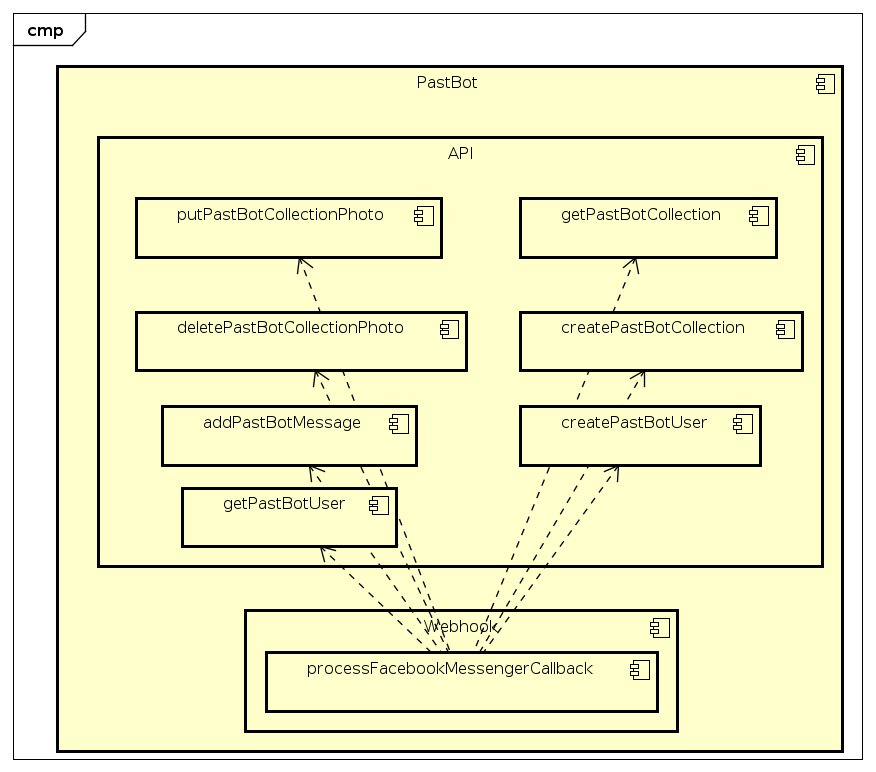
\includegraphics[scale=0.5]{design/overallDesign}
  \caption{Design generale dell'applicazione}
\end{figure}

\subsection{API}

Le classi che appartengono a questa componente hanno lo scopo di eseguire le
operazioni sulle base di dati di PastBot. Avendo uno solo scopo e una sola
responsabilità, son risultate di facile progettazione.
Per evitare ripetizioni, è riportato qui uno schema generico di una classe:

\begin{figure}[H]
  \centering
  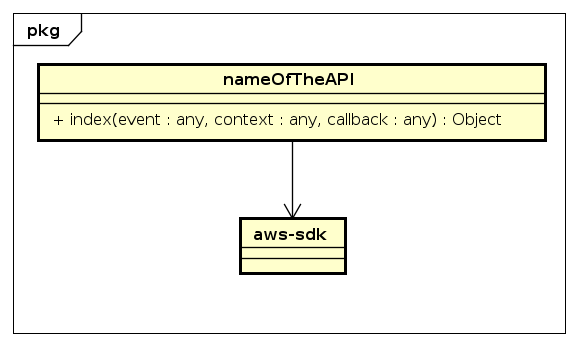
\includegraphics[scale=0.6]{design/singleAPI}
  \caption{Rappresentazione UML di una API}
\end{figure}

\label{design:api:params}
È importante segnalare come il servizio Amazon AWS Lambda passi sempre tre
parametri al metodo che andrà a invocare. Questi metodi sono:
\begin{itemize}
  \item \textbf{event}: è un oggetto in formato JSON che contiene i campi
dell'evento che viene inviato alla funzione lambda. Questi campi possono essere
definiti in maniera specifica tramite APIGateway.
  \item \textbf{context}: AWS Lambda usa questo parametro al fine di poter
ottenere informazioni a tempo di esecuzione sul tipo di funzione lambda che si
sta eseguendo.
  \item \textbf{callback}: tramite questo parametro è possibile, se necessario,
ritornare dati (in formato JSON) al chiamante o segnalare uno stato di errore
durante l'esecuzione. Essendo questo parametro opzionale, se non se ne farà uso
la risposta che si otterrà sarà un valore nullo.
\end{itemize}

\subsection{api::putPastBotCollectionPhoto}

Questa classe si occupa di aggiungere le foto inviate dall'Utente direttamente
nel database di PastBot. Essendo la \textit{privacy} un argomento molto
importante quando si trattano i dati personali degli utenti, le foto vengono
salvate indirettamente tramite il servizio \textit{Filestack}. Questo
servizio di salvataggio dati ha permesso una facile gestione dei dati degli
utenti, compreso il caricamento. Il caricamento della foto avviene inviando
l'indirizzo dell'allegato fornito da Facebook Messenger direttamente al
servizio \textit{Filestack}.


Questa classe per funzionare necessita del modulo nativo aggiuntivo
\textit{https}.

\subsection{api::getPastBotUser}

Questa classe si occupa di ritornare al chiamante le informazioni sull'utente
richieste. Viene eseguita quindi una interrogazione del database degli utenti,
in cui verrà cercato l'\textit{id} fornito nell'oggetto della richiesta. Se
l'utente viene trovato, verranno ritornate le informazioni su di esso e la
lista degli album (denominati anche \textit{collection}) creati da quell'utente
tramite il bot.
Se l'utente non è presente nella base di dati viene ritornato nell'oggetto uno
stato di errore.

\subsection{api::getPastBotCollection}

Questa classe ritorna le informazioni sull'ultimo album attivo. È necessario
fornire l'\textit{id} dell'utente per poter ottenere l'informazione.
Se viene fornito un \textit{id} non valido o non presente nella base di dati di
PastBot verrà ritornato nell'oggetto di ritorno uno stato di errore.

\subsection{api::createPastBotUser}

La classe accetta un nuovo utente e si occupa di aggiungerlo alla lista
degli utenti presenti nella base di dati di PastBot. È necessario passare un
identificativo che sia univoco per quell'utente. Se viene passato un
identificativo che è già presente nella base di dati la classe si occuperà di
ritornare al chiamante uno stato di errore.

\subsection{api::deletePastBotCollectionPhoto}

La classe si occupa di cancellare tutte le foto presenti all'interno di un
album dato. La cancellazione sancisce l'eliminazione completa dai database di
PastBot.
Lo stato della cancellazione viene riportato nell'oggetto che verrà ritornato
al chiamante.

\subsection{api::addPastBotMessage}

Questa classe ha l'incarico di salvare il messaggio ricevuto nella base di
dati. Questa funzione serve in futuro a PastBook per poter eseguire raccolta
dati e studi su di essi.

\subsection{api::createPastBotCollection}

La responsabilità di questa classe è quella di creare un nuovo album dato un
utente esistente. Se l'identificativo dell'utente non è valido verrà ritornato
un messaggio di errore, altrimenti verrà creato un nuovo album, che porterà a
sua volta un identificativo univoco.

\subsection{\textit{Webhook}}

Le classi all'interno di questo componente si occupano di gestire l'intera
interazione con gli utenti, dalla ricezione del messaggio fino alla loro
risposta. Le operazioni relative al salvataggio e recupero di informazioni sono
effettuate tramite le API, creando quindi un livello di indirettezza e una
maggiore estendibilità.
Il nome \textit{webhook} è stato dato per differenziare il bot dalle API.
Essendo infatti il bot scritto con le stesse tecnologie delle API si è dovuto
porre una differenza a livello di nome, per evitare incomprensioni.

\begin{figure}[H]
  \centering
  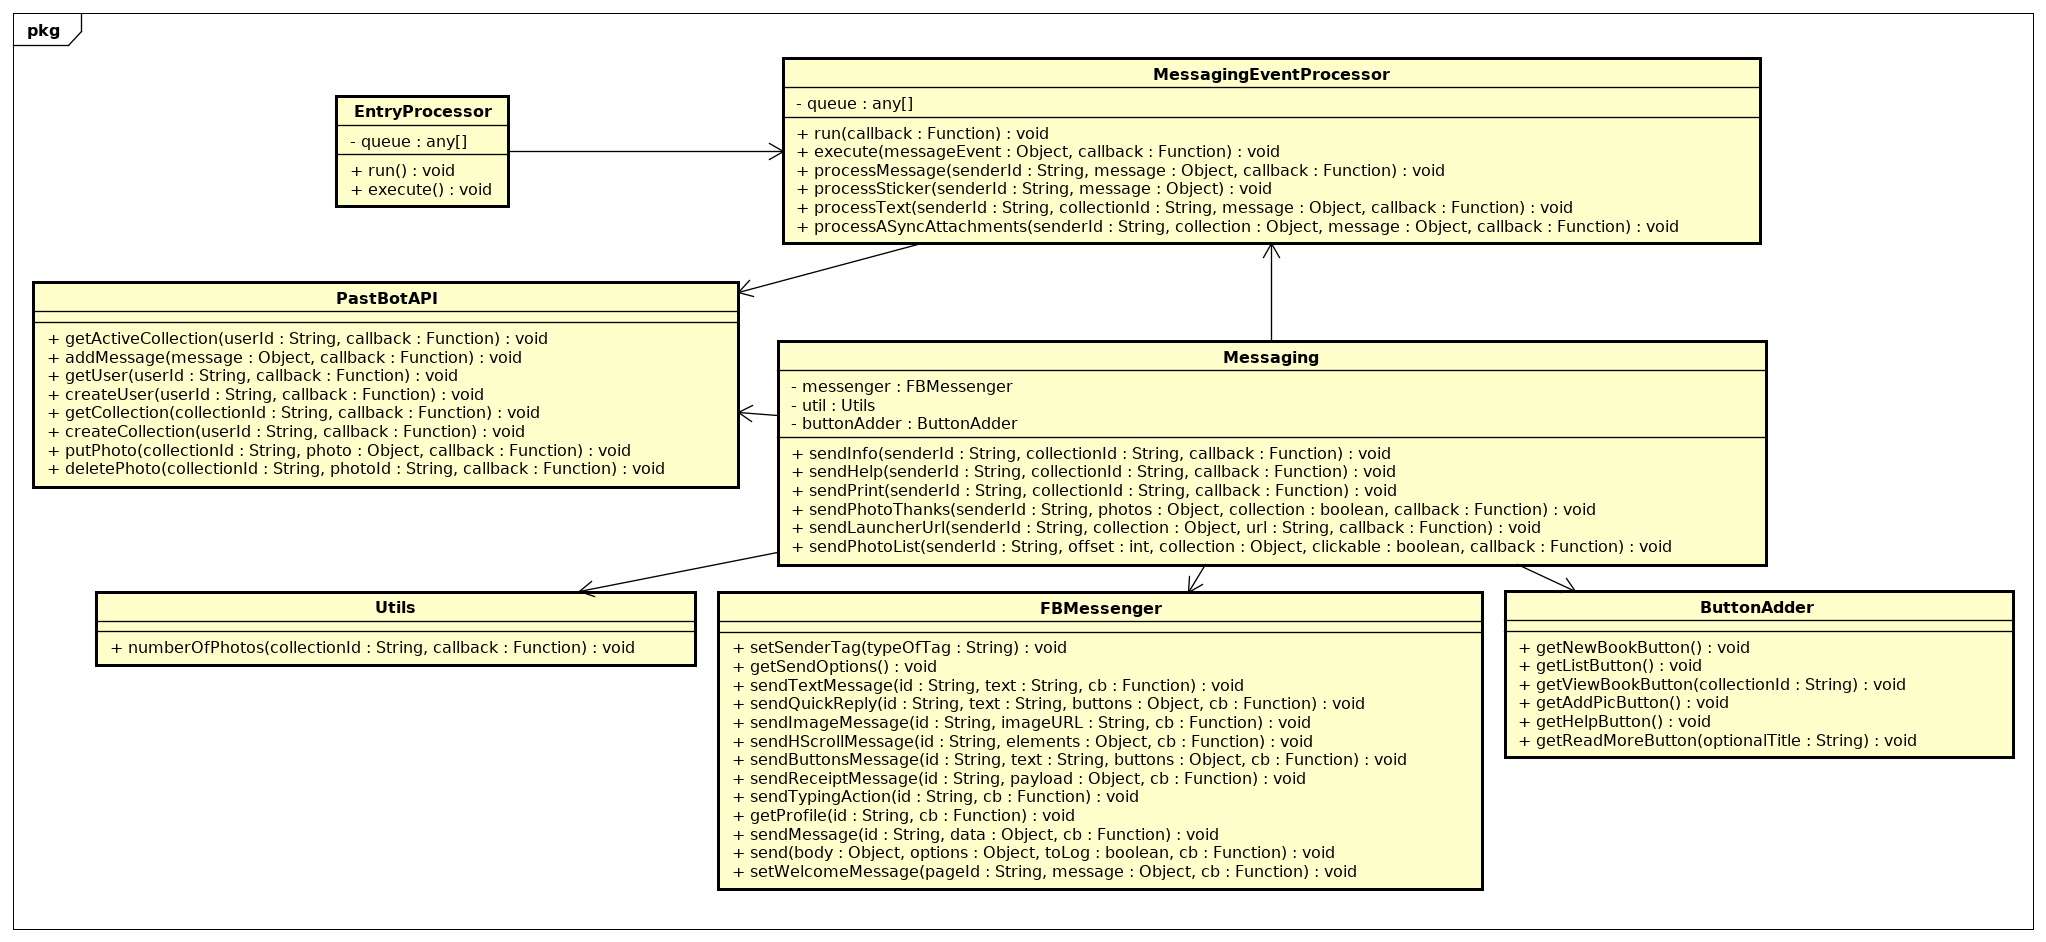
\includegraphics[scale=0.3]{design/processFacebookMessengerCallback}
  \caption{Diagramma delle classi per la parte di PastBot relativa
all'interazione con gli utenti.}
\end{figure}
